\addbibresource{reference.bib}

\chapter{Polovodičové pixelové detektory ionizujícího záření rodiny Medipix}\label{det}
Ionizující záření je lidskými smysly nedetekovatelné. Tento fakt, dal vzniku detekční technice a~metodám toto záření měřit. Tato kapitola je věnována pokročilé instrumentaci pro detekci ionizujícího záření  - hybridním polovodičovým pixelovým detektorům.

Existuje celá řada částicových pixelových detektorů (AGH\_Fermilab, Pilatus, Philips Chromaix apod.) \cite{detectors_review}, tato práce se však zabývá pouze detektory z~rodiny Medipix, které jsou vyvíjeny v~rámci stejnojmenné kolaborace Medipix\footnote{\url{http://medipix.web.cern.ch/}} v~CERN. Tato kolaborace sdružuje několik desítek vědeckých institucí a~univerzit po celém světe, mezi které patří od roku 1999 i ÚTEF ČVUT v~Praze.


\clearpage

%********************************************************************************
% Princip detekce
%********************************************************************************
\section{Princip detekce}
Činnost hybridních pixelových detektorů je založena na známém principu detekce ionizujícího záření v~polovodiči. 

Na obrázku \ref{fig:det:recomb} je znázorněn princip této detekce. V~horní části se nachází polovodičový senzor, pro který je jako materiál nejčastěji použit křemík, ale výjimkou není ani \texttt{GaAs}, či \texttt{CdTe}. Pod tímto senzorem se nachází vyčítací elektronika, která tvoří jednotlivé pixely. Jako náhradní schéma tohoto obvodu si lze představit diodu zapojenou v~závěrném směru, skrze kterou protéká jen minimální proud. 

\begin{figure}[th]
	\begin{center}
		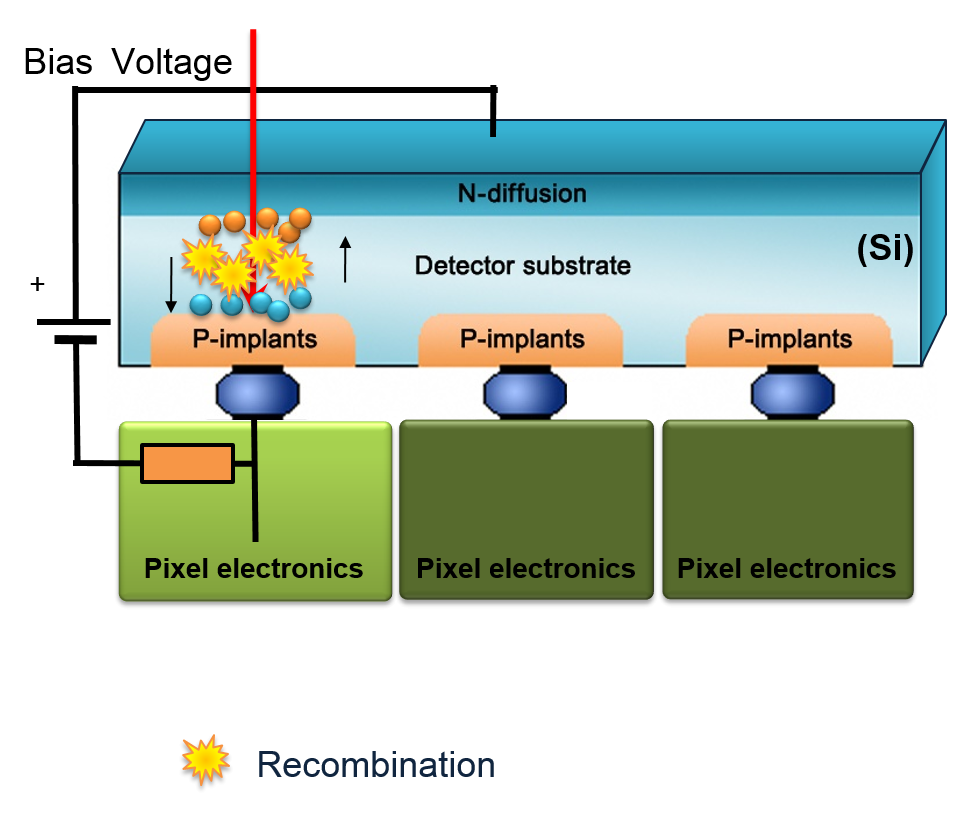
\includegraphics[width=8.5cm]{figures/det_recombination.png}
		\caption{Princip detekce ionizujícího záření (převzato z~\cite{PlatkevicDisertace}), kde červená šipka je procházející částice, žlutě jsou znázorněny elektrony, modře díry. Elektronika každého každého pixelu zpracovává napěťový pulz.}
		\label{fig:det:recomb}
	\end{center}
\end{figure}
Při vniku ionizující částice do detektoru dojde k předání části její energie detekčnímu materiálu. Vznikají elektron-děrové páry a díky lavinovému efektu dochází k otevření PN přechodu. Tím dojde ke vzniku proudového pulsu, jež je pomocí měřícího odporu převeden na napětí a dále měřící elektronikou zpracováván.

\begin{figure}[th]
	\begin{center}
		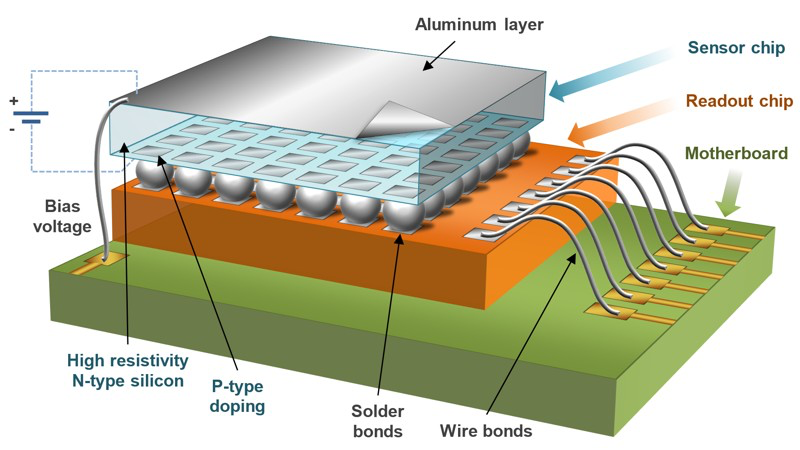
\includegraphics[width=12cm]{figures/det_chip.png}
		\caption{Struktura hybridního polovodičového pixelového detektoru rodiny Medipix (převzato z~\cite{PlatkevicDisertace})}
		\label{fig:det:chip}
	\end{center}
\end{figure}

Na obrázku \ref{fig:det:chip} je znázorněna struktura Medipix detektoru. Nahoře se nachází, polovodičový senzor (\texttt{Sensor chip}), který je spojen s~integrovaným \texttt{ASIC}\footnote{z angl. Application Specific Integrated Circuit} vyčítacím čipem (tzv. \texttt{Readout chip}) pomocí technologie zvané \texttt{bump-bonding} (na obr. \ref{fig:det:chip} jako \texttt{Solder bonds}). Odtud také pochází název "hybridní" - jedná se o spojení senzoru a~\texttt{ASIC} čipu. Každý pixel senzoru tvoří jeden PN přechod. Vyčítací čip je spojen s~další nezbytnou elektronikou (na obr \ref{fig:det:chip} znázorněnou jako \texttt{Motherboard}) pomocí tzv. \texttt{wire-bonds}. Z~této elektroniky je vyvedeno napětí na polovodičový senzor - \texttt{bias}, zajištující vyprázdnění detekčního objemu polovodičového senzoru.


%********************************************************************************
% Medipix detektory
%********************************************************************************
\newpage
\section{Detektory rodiny Medipix}\label{det:med}
Pro realizaci sítě ATLAS TPX byly použity pouze detektory typu Timepix. Pro srovnání je níže uveden stručný popis ostatních detektorů rodiny Medipix.
Do této rodiny patří především: Medipix1, Medipix2 \cite{Llopart-medipix2}, Timepix \cite{timepix}, Medipix3, nově Timepix3 \cite{timepix3} a~ další jsou ve vývoji, například Timepix2 a Dosepix. 

\begin{description}
	\item[Medipix1] Medipix1 je prvním detektorem z~této rodiny a~byl uveden v~roce 1997. Také je známy pod názvem PCC (z~angl. Photon Counting Chip). Jedná se o prototyp digitálního \texttt{CMOS}\footnote{z angl. Complementary Metal–Oxide–Semiconductor} zobrazovacího čipu, který nachází uplatnění ve vysokoenergetických fyzikálních experimentech \cite{medipix-www}. Je schopný operovat jen v~\texttt{Medipix módu} (viz \ref{det:mod}). Tento detektor má matici $64\times64$ pixelů, každý s~hranou o délce $170~\mu m$ a~celková aktivní plocha je $1,2~cm^2$. Detektor obsahuje $15$-bitový čítač, kterým umožňuje v~rámci jedné akvizice zaregistrovat až $32767$ událostí.

	\item[Medipix2] Medipix2 je přímým následníkem detektoru Medipix1. 
	%Tento model především profite z~rychlého pokroku \texttt{CMOS} technologie, díky kterému bylo možné přidání nové funkcionality a~především zmenšení velikosti pixelů. 
	Díky větší integraci \texttt{CMOS} technologie bylo možné přidat novou funkcionalitu a~zmenšit velikost pixelů.
	Detektor obsahuje matici $256\times256$ pixelů, délka hrany jednoho pixelu se zmenšila na $55~\mu m$ a~celková aktivní plocha vzrostla na $2~cm^2$.

	\item[Timepix]\label{det:tim} Tento detektor je na bázi detektoru Medipix2, prodělal však výraznou obměnu digitální části. Byla přidána synchronizační logika, která přinesla dva nové módy - TOT (měření energie) a~TOA (měření doby příletu částice), přičemž každý pixel v~jeden okamžik umožňuje měřit jen v~jednom módu
	(více o módech v~\ref{det:mod}). 
	%Další možností je nastavení globálního tresholdu\footnote{Treshold je úroveň komparačního napětí, které je porovnáváno s~aktuálním měřícím napětím na každém pixelu.Je-li tato úroveň překročena, dojde k~detekováni události.} s~lokální úpravou pro jednotlivé pixely o $4 b$. 

	\item[Medipix3] U Medipix3, byla výrazným způsobem přepracována vyčítací elektronika za cílem snížení zkreslení, způsobeném sdílením náboje mezi sousedními pixely (tento efekt je také znám pod pojmem \texttt{Charge Sharing} efekt \cite{Jakubek-radiography_and_charge_sharing}). 


	%\begin{figure}[th]
	%\begin{center}
	%	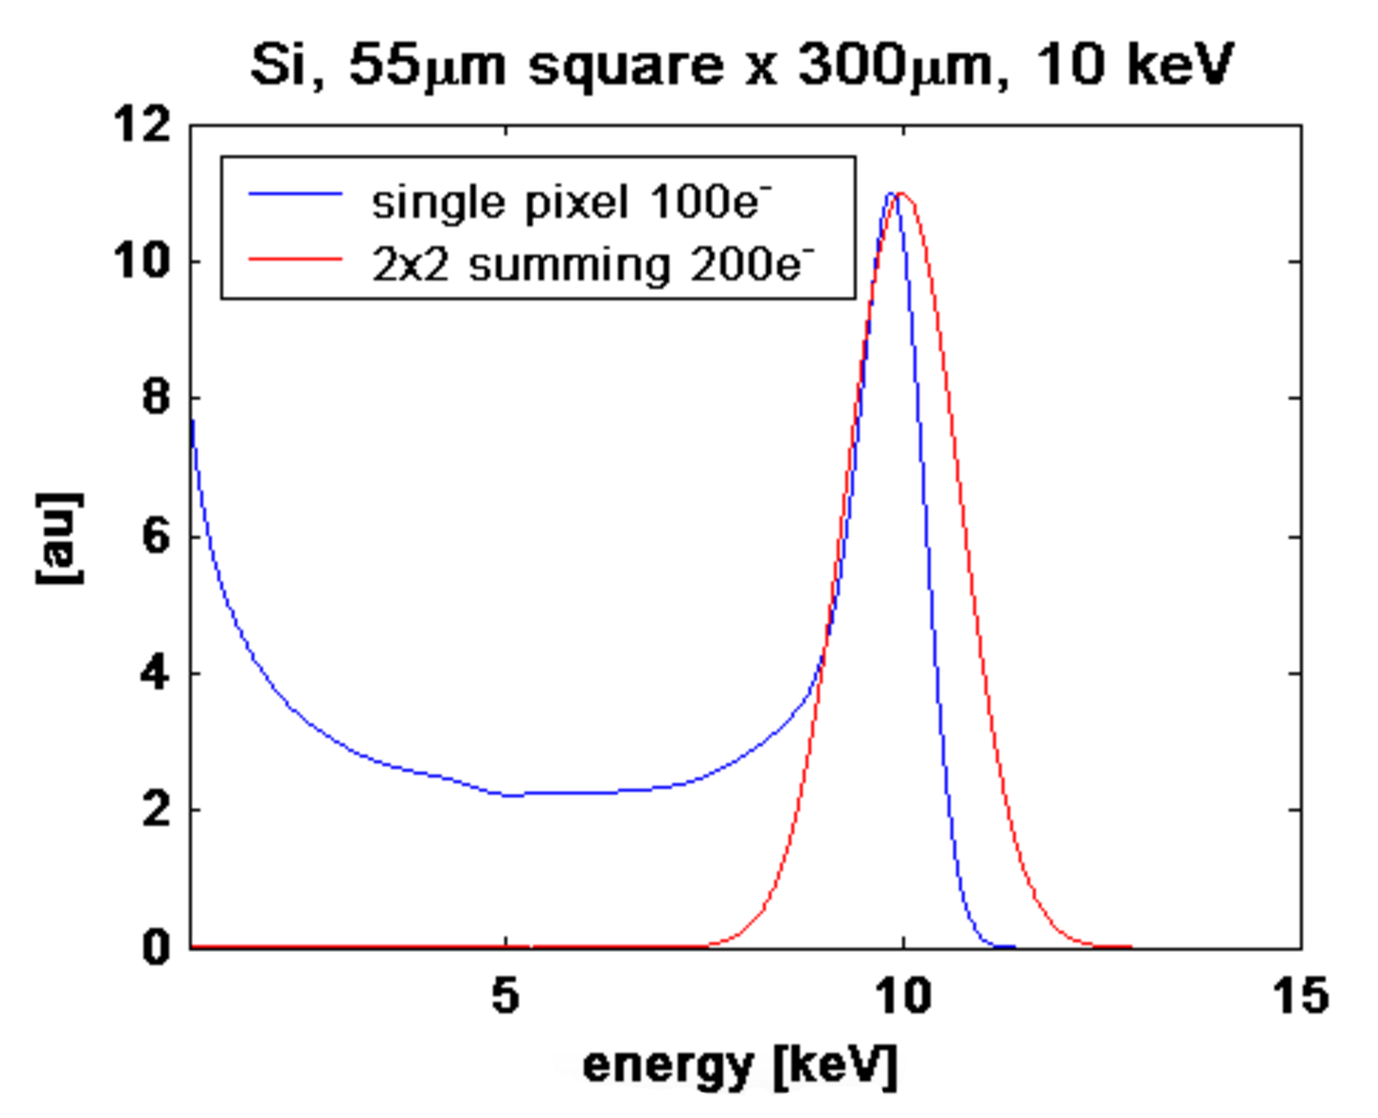
\includegraphics[width=8cm]{figures/det_charge_sharing.png}
	%	\caption{Charge Sharing Efekt (převzato z~\cite{medipix-www})}
	%	\label{fig:det:charge_sharing}
	%\end{center}
	%\end{figure}

	%Když dopadne nabitá částice na polovodičový senzor, vzniknou elektron-děrové páry, které jsou staženy nejen zasaženým pixelem, ale vetšinou i několika sousedními. To samo o sobě je žádoucí jev, problém ale nastává, když vyčtená energie sousedními pixely je nižší, než jejich prahová, potom dochází ke, již výše zmíněnému, zkreslení. 
	
	%Obrázek \ref{fig:det:charge_sharing} je demonstrací tohoto jevu. Zobrazuje histogram detekovaných energií pro jeden pixel. Když každý pixel operuje zcela nezávisle (na obrázku modře), je patrné, že daný pixel registroval i události sousedních pixelů, vzniklé \texttt{Charge Sharing} efektem. Tento problém odstraňuje \texttt{CSM} \ref{det:mod:csm} mód a~především možnost vyčítat jednotlivé události (nikoliv až celé snímky), což také odstraňuje mrtvou dobu detektoru. \texttt{CSM} mód přičte k~energii zasaženého pixelu i energii sousedních pixelů - viz obr. \ref{fig:det:charge_sharing} červeně.

	\item[Timepix3] Timepix3 vychází z detektoru Timepix, oproti kterému má tento detektor vylepšenou vyčítací logiku a~o jeden čítač na pixel více. To mu mimo jiné umožňuje měřit v~TOT a~TOA módu současně. Navíc ještě přináší \texttt{Data-driven} vyčítací mód (obdobně, jako Medipix3), který na rozdíl od \texttt{Frame-based} vyčítání minimalizuje mrtvou dobu detektoru.

\end{description}

%********************************************************************************
% Módy detektorů
%********************************************************************************
\section{Provozní módy detektorů Timepix}\label{det:mod}
V této podkapitole jsou popsány módy detektor Timepix. 
V levé části obrázku \ref{fig:det:signal_proc} je znázorněn pixel detektoru s~blokovým schématem vyčítací elektroniky. Interagující částice (na obr. znázorněna červenou šipkou) v~detekčním materiálu vyvolá proudový pulz. Ten je měřícím odporem převeden na napětí, které je dále zesilovačem (\texttt{Amplifier}) zesíleno. Toto napětí je dále porovnáno komparátorem (\texttt{Comparator}) s~komparačním napětím (tzv. tresholdem\footnote{Treshold je úroveň komparačního napětí, které je porovnáváno s~aktuálním měřícím napětím na každém pixelu. Je-li tato úroveň překročena, dojde k~detekováni události.}). 
Výsledek komparace je zpracován dle módu detektoru. Pro úplnost je třeba dodat, že \texttt{Shutter} na obr. \ref{fig:det:signal_proc} slouží pro spouštění, resp. ukončování akvizice.

\begin{figure}[th!]
	\begin{center}
		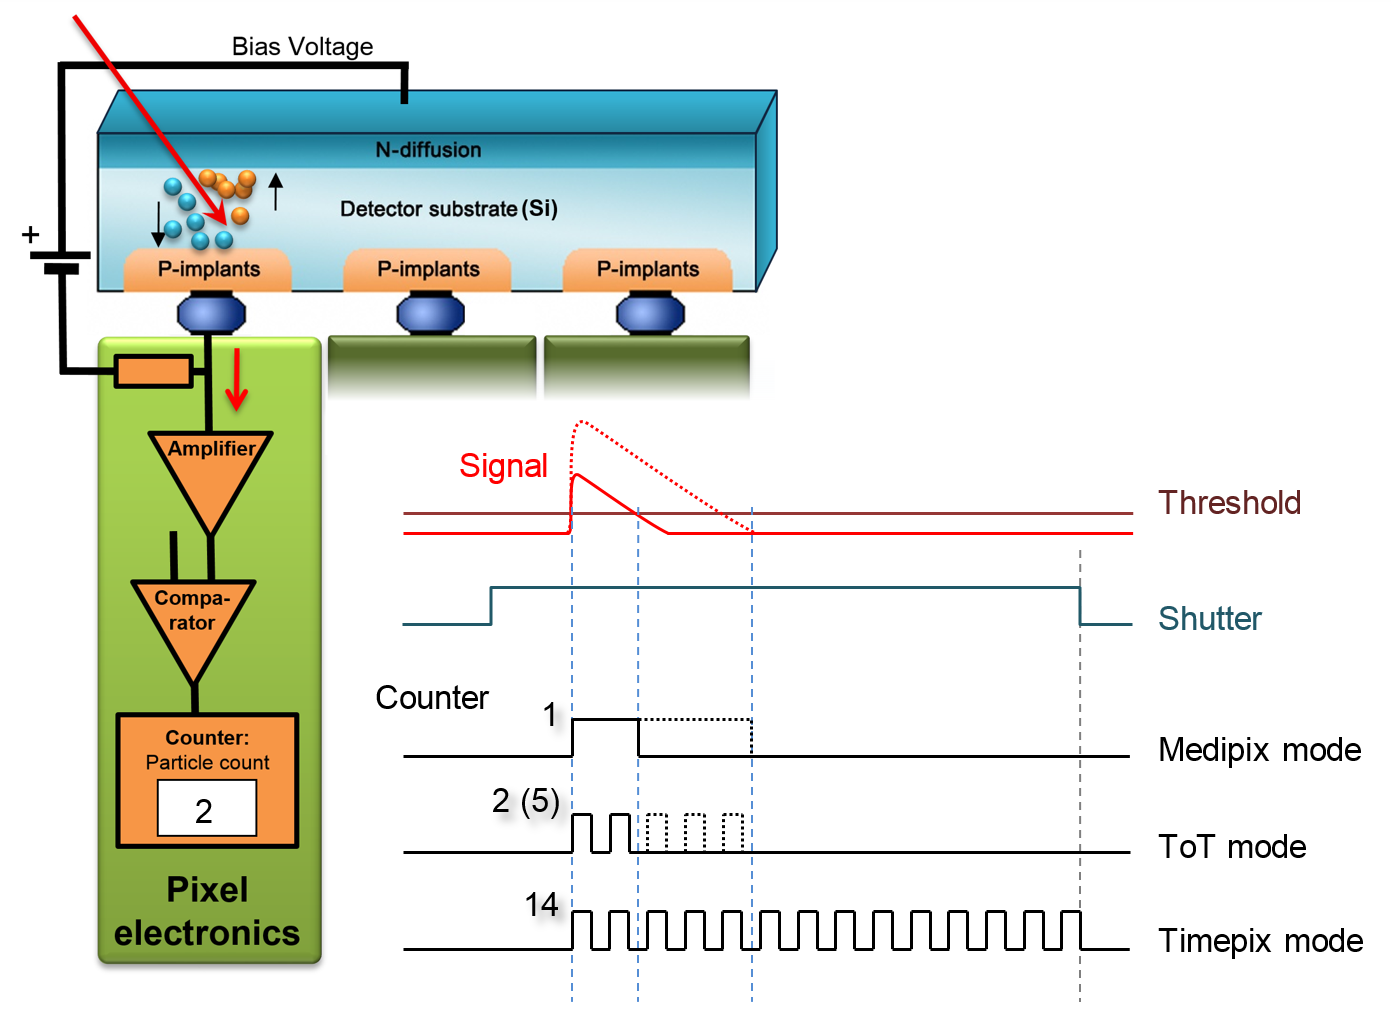
\includegraphics[width=10.75cm]{figures/det_pix.png}
		\caption{Zpracování signálu z~pohledu módu pixelu (převzato z~\cite{PlatkevicDisertace})}
		\label{fig:det:signal_proc}
	\end{center}
\end{figure}

\begin{description}
	\item[Medipix mód] Tento mód počítá počet částic, které během doby akvizice dopadly na aktivní plochu detektoru. Na obrázku \ref{fig:det:signal_proc} znázorněn, jako \texttt{Medipix mode}.
	\item[TOT (Time-Over-Treshold)] Tento mód udává, jak dlouhou dobu (v počtu hodinových cyklů měřící frekvence) bylo zesílené napětí na detektoru vyšší, než komparační (treshold). Počet těchto cyklů je ekvivalentní deponované energii částice. Tento vztach je ale nelineární a~pro získání energie z~TOT je třeba detektor kalibrovat - o tom pojednává kapitola \ref{calib}. Tento mód je podporovaný všemi Timepix detektory (ze zde uvedených detektorů).
	\item[TOA (Time-Of-Arrival)] Pixel v~tomto módu spustí svůj čítač po překročení tresholdu, čily vůči akvizičnímu času udává čas příletu částice. Tento mód je také známý pod označením \texttt{Timepix mode} a~nalézá své uplatnění především při měření koincidencí (rekonstrukce trajektorie částice, interagující s~více detektory pomocí času dopadu a~souřadnic zasažených pixelů). Tento mód je podporovaný všemi Timepix detektory (ze zde uvedených detektorů).
	%\item[SPM (Single Pixel Mode)] v~tomto módu každý pixel operuje zcela samostatně a~to v~Medipix módu.\item[CSM (Charge Summing Mode)]\label{det:mod:csm} Tento mód odstraňuje zkreslení vzniklé \texttt{Charge Sharing} efektem pomocí přičtení energie do zasaženého pixelu z~pixelů okolních. Jako zasažený pixel se určí pixel s~nejvyšší energií. Tento mód podporuje jen Medipix3 (ze zde uvedených detektorů).

\end{description}

%********************************************************************************
% FITPix
%********************************************************************************
\section{FITPix}\label{det:fitpix}
FITPix\footnote{z angl. Fast Interface for Timepix Pixel Detectors} \cite{fitpix} je vyčítací rozhraní, pracující téměř se všemi detektory rodiny Medipix, vyvíjené v~ÚTEF ČVUT v~Praze od roku 2010 - viz obr. \ref{fig:det:fitpix}. Toto rozhraní se skládá z~FPGA\footnote{z angl. Feld Programmable Gate Array} obvodu, USB 2.0 rozhraní, DAC převodníků (převodník digitálního signálu na analogový), ADC převodníků (převodník analogového signálu na digitální) a~z obvodů generující napětí pro polovodičový senzor (tzv. bias). Toto zařízení umožňuje plnohodnotné ovládání připojeného detekčního čipu, včetně nastavování měřící frekvence, tresholdu, řízení shutteru (sloužícího pro ovládání akvizice, viz \ref{det:mod}) apod. Také přináší možnost ovládat shutter pomocí hardwarového trigger signálu pro měření s~více detektory současně, resp. pro jejich synchronizaci.

\begin{figure}[th!]
	\begin{center}
		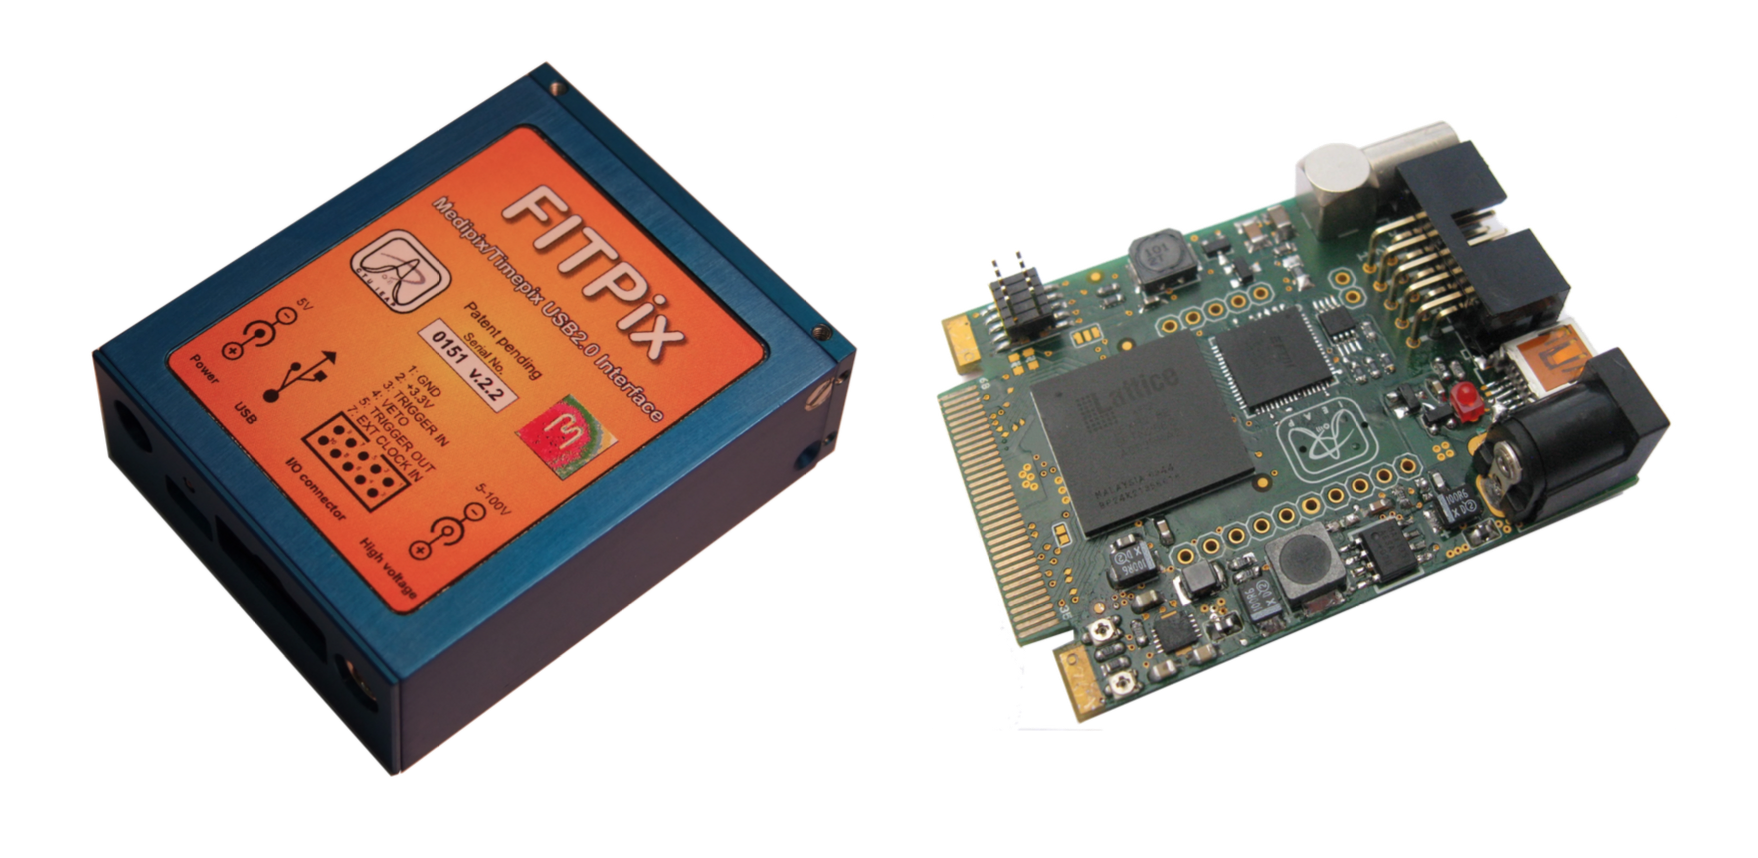
\includegraphics[width=11cm]{figures/fitpix.png}
		\caption{FITPix}
		\label{fig:det:fitpix}
	\end{center}
\end{figure}

Tato architektura s~FPGA byla použita především z~důvodu dosažení vyšších datových toků a~také vyšší radiační odolnosti, které by za použití konvenčních mikroprocesorů nemohlo být dosaženo. Další výhodou je menší počet aktivních prvků, což se projeví krom spotřeby i na nižších tepelných ztrátách. Tento parametr je velice důležitý, především pro nasazení ve vakuu.

%********************************************************************************
% Pixelman
%********************************************************************************
\section{Pixelman}\label{det:pixelman}
Pixelman \cite{pixelman} je softwarový balík, vyvíjený v~ÚTEF ČVUT v~Praze, sloužící pro řízení detektorů z~rodiny Medipix pomocí vyčítacího rozhraní FITPix \ref{det:fitpix}. Tento software umožňuje akvizici dat, jejich vizualizaci a~následnou analýzu.

Jedná se o vysoce modulární systém, který mimo jiné umožňuje rozšíření své funkcionality o pluginy, které mají přístup k~funkcím, poskytovaným jádrem Pixelmanu. Dokonce každý plugin může zaregistrovat své funkce, takže i ostatní pluiny mohou využívat jeho funkcionalitu. Jsou podporovány pluginy, vyvinuté v~jazycích Java, C/C++ a~Python. Na obrázku \ref{fig:det:pixelman} je znázorněna softwarová architektura Pixelmana.

\begin{figure}[th!]
	\begin{center}
		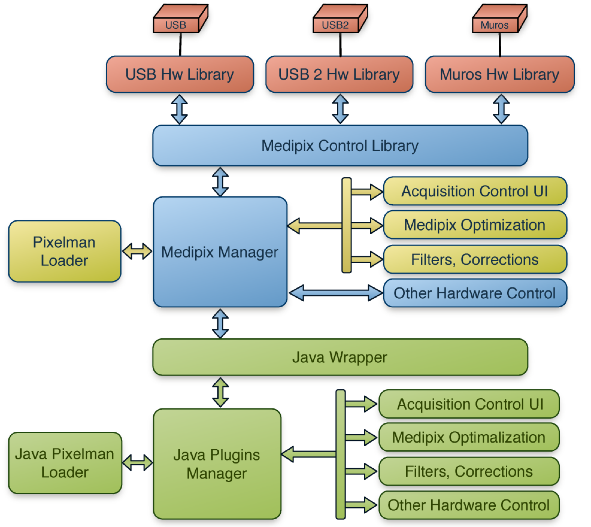
\includegraphics[width=10.25cm]{figures/pixelman.png}
		\caption{Pixelman - sw architektura (převzato z~\cite{pixelman})}
		\label{fig:det:pixelman}
	\end{center}
\end{figure}




